\apendice{Especificación de diseño}
\section{Introducción}
En el apéndice anterior se detallaron los requisitos del software. El siguiente paso es mostrar las especificaciones de diseño. En este apéndice se explicarán los motivos para las soluciones tomadas en relación al diseño de este programa. 
El diseño del software recoge las cuestiones relativas a la gestión de los datos y su presentación, a la división de las partes del código en otros módulos y cómo se estructura su funcionamiento. En definitiva, se expone cómo se estructura el software arquitectónicamente.

\subsection{Ámbito del software}
El software desarrollado permite al usuario controlar motores y ser conocedor de la temperatura ambiente de la zona en la que esta situado, mediante el manejo de un sistema empotrado que se comunica por red con otros SE que, a su vez, interactúan con los motores o medios de interacción con las personas como pantallas LCD o leds. El software es específico, como es habitual en el ámbito de los SE, para la planta piloto presentada. La interacción con el usuario es muy sencilla y se realiza mediante la pulsación de botones y el giro de potenciómetros.


\section{Diseño de datos}
La base del proyecto es la comunicación entre sistemas empotrados. En esta comunicación se envían comandos que serán recibidos y gestionados por otros sistemas embebidos. Los comandos son cadenas de caracteres que se procesarán por software hasta activar la acción que el SE debe realizar. Veamos el proceso en detalle.

\subsection{Transferencia de los comandos.}
La comunicación entre placas para enviar y recibir comandos se implementa siguiendo el protocolo TCP Transmision Control Protrocol. Este modelo se encarga de realizar la comunicación estableciendo la conexión. Para realizar esta labor enviara unos comandos de sincronización \cite{establecerConexionTCP} tal y como veremos en la Figura \ref{establecimientoConexionTcp}

\begin{figure}[!h]
	\centering
	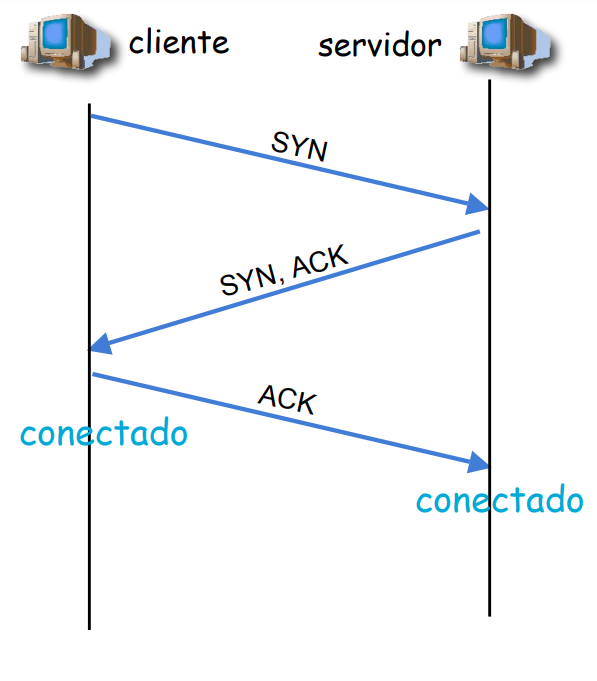
\includegraphics[width=0.6\textwidth]{establecerConexionTCP}
	\caption{Establecimiento de conexion TCP \extranjerismo{(3 way Handshake)}}\label{establecimientoConexionTcp}
\end{figure}

Los pasos a seguir para establecer la conexión son:
\begin{enumerate}
\item El cliente envía un segmento al servidor solicitando la conexión. Este segmento no contiene datos, tan solo la cabecera. A este segmento se le conoce como `SYN'.
\item El servidor responde al segmento confirmando \extranjerismo{`ACKnowledgement'} la recepcion del `SYN'. Este segmento indica al cliente el deseo de establecer conexión (SYN). Al igual que el segmento anterior, no contiene datos, solo cabecera.
Tras ejecutar este proceso de inicialización, los comandos se envían encapsulados en los segmentos TCP.
\item Por último, el cliente envía confirmación al `SYN' enviado por el servidor y se establece la conexión.
\end{enumerate}

Una vez establecida la conexión, cliente y servidor pueden intercambiar segmentos con datos. Para interrumpir esa conexión se deben enviar los paquetes que se muestran en la \ref{cierreConexionTcp}

\begin{figure}[!h]
	\centering
	\includegraphics[width=0.6\textwidth]{CierreConexionTCP}
	\caption{Cierre de conexión TCP.}\label{cierreConexionTcp}
\end{figure}


Los pasos siguientes describen como se interrumpe la conexión TCP:
\begin{enumerate}
\item Tanto el servidor como el cliente pueden tratar de terminar la conexión. Para ello se comienza enviando un comando a la otra parte llamado ´FIN' sin datos.
\item La parte que recibe el comando debe confirmar su recepción enviando un (ACK). La parte que envió el comando FIN ya no puede enviar más datos. 
\item La misma parte que recibió el comando `FIN', envía un segmento sin datos, solicitando el cierre.
\item Por último, el receptor del segundo segmento `FIN', debe confirmar la recepción del segmento. Por si ese último `ACK' se perdiera, el emisor del mensaje debe esperar un tiempo, incluso en algunas ocasiones podría tener que volver a enviarlo.
\end{enumerate}

Con estos cuatro pasos se cerraría una conexión TCP.

\subsection{Envío y recepción de comandos}
Todos los casos de uso para los que se puede utilizar la planta piloto se realizan mediante el envío de comandos. Desde la placa maestro, el usuario utiliza los botones y potenciómetros para configurar el envío de una petición a las otras placas que están conectadas mediante red. Una vez enviado el comando, una de las dos placas esclavo. El primer paso es descomponer el comando en distintas variables que procesarán hasta llegar a enviar una petición a los motores o reenviar información a la placa maestro o mostrarla por pantalla, en ambas se tramita el comando de la misma manera. 

Los comandos tienen el siguiente formato ``****/****/****/''. Cada una de las barras hace de separador para guardar la información en cada variable, la longitud de los caracteres puede variar dependiendo del comando que se quiera enviar. Los comandos están determinados en el propio software y no pueden variar puesto que el usuario no los escribe tan solo maneja los botones de las placas para elegir cual mandar.

En la siguiente \ref{tabla:Comandos} vamos a ver cuáles son los comandos existentes en este proyecto

\tablaSmallSinColores{Lista de comandos}{c c c c l}{Comandos}
{\multicolumn{1}{l}{CMD}& Arg1& Arg2& Arg3& Descripción\\}
{
Set Speed 1 & uart/ & Vel1/ &  0/ & El motor 1 gira hacia la izquierda\\
     -      & uart/ & Vel1/ & 128/ & El motor 1 se para\\
     -      & uart/ & Vel1/ & 255/ & El motor 1 gira hacia la derecha\\ \hline
Set Speed 2& uart/ & Vel2/ &  0/  & El motor 2 gira hacia la izquierda\\
     -      & uart/ & Vel2/ & 128/ & El motor 2 se para\\
     -      & uart/ & Vel2/ & 255/ & El motor 2 gira hacia la derecha\\ \hline
Parada de & uart/ & stop/ & - & Ambos motores se paran \\
emergencia & & & & \\ 
\hline
Obtener& temp/ & `X'/ & - & El maestro envía la temperatura\\
temperatura & & & & envía la temperatura\\ 
\hline
Obtener & uart/ & GVel1/ & - & El maestro pide la\\
velocidad 1 & & & & velocidad del motor A\\
Obtener & uart/ & GVel2/ & - & El maestro pide\\
velocidad 2 & & & & la velocidad del motor B\\ 
\hline
Obtener & g\_vel/ & mot1/ & `X'/ & Esclavo devuelve la velocidad del\\
velocidad 1a & & & & motor A.  `X' podrá ser 0, 128, 255\\
Obtener & g\_vel/ & mot2/ & `X'/ & Esclavo devuelve la velocidad del\\
velocidad 1b & & & & motor B.  `X' podrá ser 0, 128, 255\\
}

\subsubsection{Implementación de la conexión con lwIP}

LwIP incluye la librería Netconn API \cite{nonGNU} nos facilita varias funciones que podemos utilizar para el establecimiento de una conexión, envío de datos e interrupción de la conexión. Todos los SE de la planta piloto cuentan con recepción de comandos \extranjerismo{(Listener)} y con envío de comandos \extranjerismo{(Writer)}. Los comandos utilizados para la recepción de datos en este proyecto son:
\begin{itemize}
\item netconn\_new. Crea una conexión.
\item netconn\_bind. Vincula un netconn a una dirección IP y un puerto local específicos.
\item netconn\_listen. Establece una conexión TCP en modo de escucha.
\item netconn\_accept. Acepta una conexión entrante en una conexión TCP de escucha
\item netconn\_recv. Recibir datos (en forma de un netbuf que contiene un búfer de paquetes) de un netconn.
\item netconn\_delete. Cierra una `conexión' netconn y libere sus recursos.
\end{itemize}

Por otro lado, para el envío de datos se han usado las siguientes funciones:
\begin{itemize}
\item netconn\_new. Crea una conexión.
\item netconn\_connect. Conecte un netconn a una dirección IP y un puerto remotos específicos.
\item netconn\_write. Envía datos en un TCP netconn conectado
\item netconn\_delete. Cierra una `conexión' netconn y libere sus recursos.
\end{itemize}

Estos son las funciones que se han utilizado en el software, sin embargo, existen más funciones en Netconn API para adaptarse a otras necesidades, \cite{NetconnAPI}.

\section{Diseño arquitectónico}
Según el estándar IEEE 42010\-2011 \cite{IEEE291482018} la arquitectura del software se define como `conceptos fundamentales o propiedades de un sistema en su entorno encarnados por sus elementos, relaciones, y en los principios de su diseño y evolución'. Dicho esto, veamos de manera más especifica el diseño arquitectónico de este sistema de SE.

\subsection{Diseño arquitectónico del SE}
Una de las grandes cualidades de los sistemas empotrados es que se pueden relacionar con el entorno mediante sensores. Esto hace que el software se pueda reajustar según los datos obtenidos por estos sensores. 

En este caso como ya sabemos, la gestión de las tareas se realiza en tiempo real, lo cual requiere una configuración en las tareas algo más compleja que si dispusiéramos de un SE cíclico. Se deben asignar prioridades y es necesario utilizar un software que nos ayude en esta gestión, en este caso hemos utilizado FreeRtos.

Una buena práctica para este tipo de sistemas es la utilización de interrupciones, así evitamos que el programa tenga que realizar sondeos del entorno constantemente. Las interrupciones se pueden programar para activarse al pulsar un botón o al detectar algún cambio en el entorno mediante los sensores. En ese momento se activa la interrupción y se pone en marcha la tarea correspondiente.

Una alternativa a utilizar un RTOS es la utilización de una programación cíclica. El algoritmo cíclico recorre todas las tareas una a una y cuando termina con la última vuelve a empezar. Se le puede añadir un periodos, de ejecución máximos, conocidos como 'Quantum', consiguiendo así que una tarea no este en ejecución durante un periodo de tiempo excesivo. 
Sin embargo, como se comentó anteriormente, se decidió utilizar FreeRTOS. Esta decisión se basa en el bajo tiempo de respuesta que proporciona el SO. Mediante las prioridades elegimos además que tarea debe ejecutarse antes que otras, aportando flexibilidad a la ejecución del programa.

\begin{figure}
 \centering
  \subfloat[Cíclico]{
   \label{ciclico}
    \includegraphics[width=0.3\textwidth]{bucleCiclico.png}}
  \subfloat[RTOS]{
   \label{fig:rtos}
    \includegraphics[width=0.2\textwidth]{bucleRtos.png}}
 \caption{Distintos algoritmos para la ejecución de un SE}
 \label{tiposProg}
\end{figure}

\subsubsection{Tareas programadas}
Vamos a ver que tareas se inicializan en la tercera parte de la Figura \ref{fig:rtos} para la correcta ejecución del software presentado.

\subparagraph{Tareas del maestro}
Las tareas que incluye el software maestro son:
\begin{enumerate}
    \item Init\_IP. Esta tarea se encarga de Inicializar la pila TCP/IP utilizando lwIP y establecer una IP fija según la dirección MAC de la placa. De esta manera podremos comunicarnos con otras placas en red.
    \item Writer\_Thread. Se encarga de enviar los comandos que configura el usuario a las placas esclavo.
    \item Listener\_Thread. Se encarga de establecer las conexión para poder recibir datos mediante un puerto y una IP determinados.
    \item Temp\_thread. Se encarga de conseguir el voltaje del sensor de temperatura y enviárselo a la placa esclavo.
\end{enumerate}

\subparagraph{Tareas del esclavo}
Las tareas que incluye el software esclavo son:
\begin{enumerate}
    \item init\_ip. Cumple las mismas funciones que en el maestro.
    \item listener\_thread. Realiza la misma tarea que en el maestro.
    \item uart\_task. Recibe el comando del SE maestro y se comunica con los motores enviando los bytes correspondientes al comando recibido.
    \item temp\_task. Recibe el comando del SE maestro con el voltaje del sensor de temperatura. Se encarga de calcular la temperatura y mostrarla por pantalla.
\end{enumerate}

\subsection{Diseño del uso de la placa}
Los sistemas embebidos tienen como una de sus características principales la sencilla interacción con las personas, por ello se ha tratado de que el usuario que requiera utilizar el sistema, lo haga desde un solo SE y mediante botones y luces led pueda saber si envió la información. Su uso es simple y cuenta además tanto con leds en las tres placas como con una pantalla LCD que muestra un aviso al recibir un comando además de encender los leds de la placa en rojo y verde según este disponible para recibir un nuevo comando o este gestionando uno en ese momento.


\section{Diseño procedimental}
En esta sección vamos a ver un diagrama de secuencia \ref{diagSecc} que muestra las interacciones entre los SE desde que el usuario configura y manda un comando hasta que se recibe y gestiona ese comando. 

\begin{figure}%
    \begin{center}%
    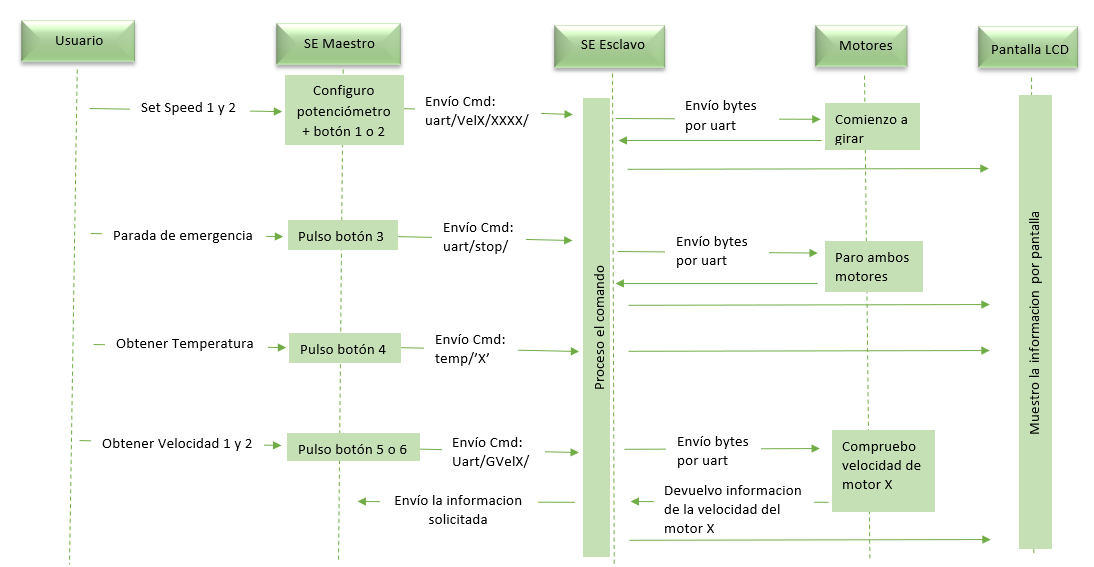
\includegraphics[angle=90]{diagSec}%
    \caption{Diagrama de secuencia de los casos de uso.}%
    \label{diagSecc}%
 \end{center}%
 \end{figure}%